\problemname{Bonsai}
Många gillar att odla bonsaiträd för att de säger att det är "svårt" och "harmoniskt". Det är inte därför Torstina odlar bonsaiträd. Hon vill bara sälja dem och tjäna massa pengar så att hon kan köpa massa kirimojor. Hon har precis planterat en ny knöl och är väldigt sugen på kirimojor. Hon undrar därför hur många år hon måste vänta innan hon har ett bonsaiträd som hennes kund önskar.

Bonsaiträd har $N$ knölar och $N-1$ grenar. Knölarna är numrerade från 0 till $N-1$. Alla bonsaiträd börjar med en liten knöl som man stoppar ner i jorden. Varje år växer det ut en ny gren från varje knöl och i dess ände bildas en ny knöl. Man kan också klippa av grenar från trädet när som helst. Hon påminner dig om att det inte spelar någon roll var roten sitter i trädet. 

Givet bonsaiträdet kunden önskar, hur många år måste Torstina vänta innan hon har odlat ett exakt likadant träd?

\section*{Indata}
Den första raden innehåller ett heltal $N$ ($2 \leq N \leq 10^5$), antalet knölar i kundens bonsaiträd.
De följande $N$ raderna beskriver bonsaiträdet enligt följande:
På rad $i$ står först ett heltal $0 < m_i < N$, antalet grenar som går ut från knöl $i$. Därefter följer $m_i$ heltal, knölarna som sitter ihop med knöl $i$. 

\section*{Utdata}
Ett heltal $A$, antalet år det tar för Torstina att odla bonsaiträdet hennes kund önskar.

\section*{Poängsättning}
Din lösning kommer att testas på en mängd testfallsgrupper.
För att få poäng för en grupp så måste du klara alla testfall i gruppen.

\noindent
\begin{tabular}{| l | l | p{12cm} |}
  \hline
  Grupp & Poängvärde & Gränser \\ \hline
  $1$   & $9$        & $m_i\leq 2$, det är bäst att börja odla trädet i nod 0. \\ \hline
  $2$   & $11$       & $m_i \leq 3$, det är bäst att börja odla trädet i nod 0. \\ \hline
  $3$   & $18$       & $A \leq 15$, det är bäst att börja odla trädet i nod 0. \\ \hline
  $4$   & $22$       & Det är bäst att börja odla trädet i nod 0. \\ \hline
  $5$   & $12$       & $N \leq 250$. \\ \hline
  $6$   & $28$       & Inga ytterligare begränsningar. \\ \hline
\end{tabular}


\section*{Förklaring av exempelfall 1}
Vi kan odla trädet på 2 år om vi låter det växa enligt bilden nedan. 

\begin{figure}[h]
	\centering
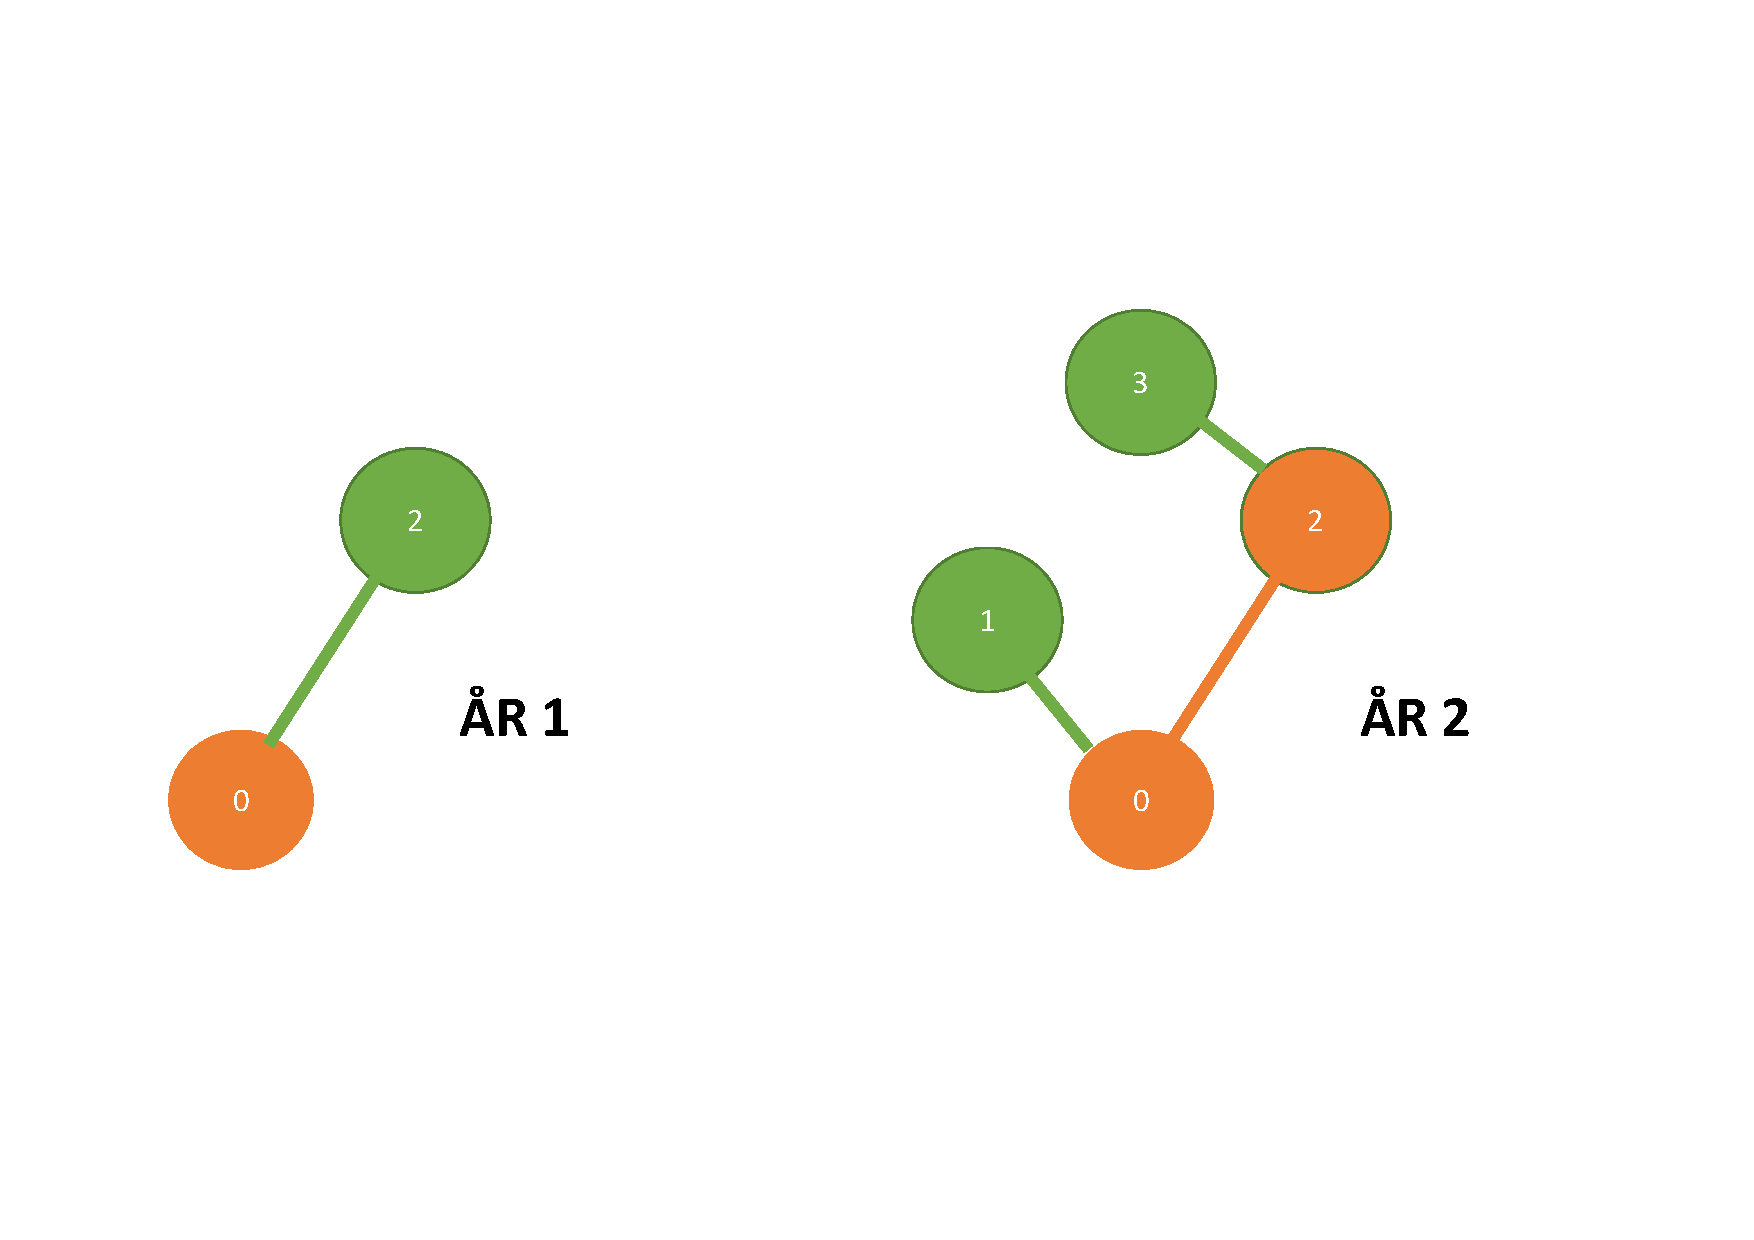
\includegraphics[width=0.5\textwidth]{Bonsai_tree}
\caption{Ett av de två sätten man kan odla bonsaiträdet i sample 1 på två år.}
\end{figure}
